%
% cholesky.tex -- Cholesky-Zerlegung
%
% (c) 2009 Prof Dr Andreas Mueller, Hochschule Rapperswil
%
\section{Cholesky-Zerlegung}
\rhead{Cholesky-Zerlegung}
\index{Cholesky-Zerlegung}
\index{Zerlegung!Cholesky}
Kann man aus einer Matrix die Wurzel ziehen? Was wäre das überhaupt?
Aus einer Diagonalmatrix mit positiven Diagonalelementen kann man offenbar
die Wurzel ziehen, in dem man die Wurzel aus den Diagonalelementen zieht.
Negative Diagonalelemente machen dies unmöglich.
Man muss also auf jeden
Fall fordern, dass die Matrix in einem gewissen Sinn positiv ist.

\begin{definition}
Eine symmetrische Matrix $A$ heisst positiv definit, falls $v^tAv>0$ für
alle Vektoren $v\ne 0$.
\end{definition}

Im Abschnitt \ref{section:ueberbestimmt} haben wir eine Anwendung
kennengelernt, in der ein Gleichungssystem der Form
\[
A^tAx=A^t b
\]
gelöst werden musste.
Die Matrix $A^tA$ ist genau von der hier
beschriebenen Art: symmetrisch und positiv definit.
Es ist nämlich
\[
v^tA^tAv=(Av)^tAv=(Av)\cdot (Av)=|Av|^2> 0
\]
falls $A$ regulär, wie für positiv definite Matrizen gefordert.

Für positiv definite symmetrische Matrizen gibt es eine Quadratwurzel
im Sinne des folgenden Satzes:
\begin{satz}[Cholesky-Zerlegung]
\index{Cholesky-Zerlegung}
\index{Zerlegung!Cholesky}
Ist $A$ eine symmetrische positiv definite Matrix, dann gibt es genau eine
untere Dreiecksmatrix $L$ mit $A=LL^t$.
\end{satz}

Anstelle eines Beweises zeigen wir einen Algorithmus, mit dem man die Matrix
$L$ konstruieren kann.
Das Verfahren startet mit einer positiv definiten
symmetrischen $n\times n$-Matrix $A$.
Gesucht wird eine untere Dreiecksmatrix $L$
mit $A=LL^t$.
Die Matrix $L$ kann man symbolisch in der Form 
\[
L=\left(
\begin{tabular}{>{$}c<{$}|>{$}c<{$}>{$}c<{$}>{$}c<{$}}
l_{11}&&0&\\
\hline
&&&\\
l&&L'&\\
&&&
\end{tabular}
\right)
\]
Darin ist $l'$ ein $n-1$-dimensionaler Spaltenvektor und $L'$ eine
untere Dreiecksmatrix mit $n-1$ Zeilen und Spalten.
Wir wollen $LL^t$ mit $A$ vergleichen, und unterteilen deshalb auch die
Matrix $A$ nach dem gleichen Muster
\[
A=\left(
\begin{tabular}{>{$}c<{$}|>{$}c<{$}>{$}c<{$}>{$}c<{$}}
a_{11}&&a^t&\\
\hline
&&&\\
a&&A'&\\
&&&
\end{tabular}
\right).
\]
Dann bekommen wir für $LL^t$:
\[
LL^t=
\left(
\begin{tabular}{>{$}c<{$}|>{$}c<{$}>{$}c<{$}>{$}c<{$}}
l_{11}&&0&\\
\hline
&&&\\
l&&L'&\\
&&&
\end{tabular}
\right)
\left(
\begin{tabular}{>{$}c<{$}|>{$}c<{$}>{$}c<{$}>{$}c<{$}}
l_{11}&&l^t&\\
\hline
&&&\\
0&&L'^t&\\
&&&
\end{tabular}
\right)
=
\left(
\begin{tabular}{>{$}c<{$}|>{$}c<{$}>{$}c<{$}>{$}c<{$}}
l_{11}^2&&l_{11}l^t&\\
\hline
&&&\\
l_{11}l&&ll^t+L'L'^t&\\
&&&
\end{tabular}
\right)
\]
Daraus können wir ablesen, dass 
\begin{align*}
a_{11}&=l_{11}^2   &\Rightarrow&&l_{11}&=\sqrt{a_{11}}\\
     a&=l_{11}l    &\Rightarrow&&     l&=\frac1{\sqrt{a_{11}}}a\\
    A'&=ll^t+L'L'^t&\Rightarrow&&L'L'^t&=A'-ll^t
\end{align*}
Um $L$ zu finden, muss also nur noch eine Zerlegung von $A'-ll^t$
finden.
Damit wurde das $n$-dimensionale Problem auf ein $n-1$-dimensionales
Problem reduziert.
Durch Wiederholung dieses Schrittes gelangt man am Schluss
zu einem eindimensionalen Problem, also dem Problem, die Wurzel aus einer
positiven Zahl zu ziehen.

\begin{beispiel}
Man finde die Cholesky-Zerlegung der Matrix
\[
A=\begin{pmatrix}
9&3&3\\
3&17&21\\
3&21&107
\end{pmatrix}.
\]
Der erste Schritt leitet daraus ab, dass
\begin{align*}
l_{11}&=3,&
l&=\frac13\begin{pmatrix}3\\3\end{pmatrix}=\begin{pmatrix}1\\1\end{pmatrix},&
ll^t&=\begin{pmatrix}1&1\\1&1\end{pmatrix},&
A'-ll^t&=\begin{pmatrix}16&20\\20&106\end{pmatrix}
\end{align*}
Bis jetzt ist bekannt, dass
\[
L=\begin{pmatrix}
3&0&0\\
1&?&?\\
1&?&?
\end{pmatrix}
\]
Für den unbekannten Teil wird jetzt der gleiche Algorithmus auf
die Matrix $A'-ll^t$ angewendet.
Im zweiten Schritt muss jetzt die Matrix $A'-ll^t$ zerlegt werden.
Wir rezyklieren die Bezeichnungen aus dem ersten Schritt, und
bekommen
\begin{align*}
l_{11}&=4,&
l&=\frac14\begin{pmatrix}20\end{pmatrix}=\begin{pmatrix}5\end{pmatrix},&
ll^t&=\begin{pmatrix}25\end{pmatrix},&
A'-ll^t&=\begin{pmatrix}81\end{pmatrix}
\end{align*}
Damit ist jetzt von $L$ bekannt:
\[
L=\begin{pmatrix}
3&0&0\\
1&4&0\\
1&5&?
\end{pmatrix}
\]
Für das fehlende Element muss jetzt nur noch die Cholesky-Zerlegung
einer $1\times 1$-Matrix bestimmt werden, dies ist aber die 
Quadratwurzel.
Somit ist
\[
L=
\begin{pmatrix}
3&0&0\\
1&4&0\\
1&5&9
\end{pmatrix}
,\quad\text{Kontrolle:}\;
\begin{pmatrix}
3&0&0\\
1&4&0\\
1&5&9
\end{pmatrix}
\begin{pmatrix}
3&1&1\\
0&4&5\\
0&0&9
\end{pmatrix}
=\begin{pmatrix}
9&3&3\\
3&17&21\\
3&21&107
\end{pmatrix}=A.
\]
\end{beispiel}

{\small
Unsere Beschreibung des Algorithmus für die Cholesky-Zerlegung ist in
einem Punkt unvollständig.
Woher wissen wir, dass $A'-ll^t$ positiv
definit ist? Dies ist ja die Voraussetzung, dass der Algorithmus
überhaupt angewendet werden kann.

Wir wissen, dass $A$ und $A'$ positiv definit sind.
Für jeden $n-1$-dimensionalen Vektor $v$ können wir einen Vektor
\[
\tilde v=\left(
\begin{tabular}{c}
$\alpha$\\
\hline
$\mathstrut$\\
$v$\\
$\mathstrut$
\end{tabular}
\right)
\]
bilden.
Nach Voraussetzung ist $v^tA'v>0$ und $\tilde v^tA\tilde v>0$.
Wir möchten nachrechnen, dass $v^t(A'-ll^t)v>0$ gilt, das würde bedeuten,
dass $A'-ll^t$ positiv definit ist.
Es ist
\begin{align*}
0\ge
\tilde v^tA\tilde v
&=
\left(
\begin{tabular}{>{$}c<{$}|>{$}c<{$}>{$}c<{$}>{$}c<{$}}
\alpha&&v^t&
\end{tabular}
\right)
\left(
\begin{tabular}{>{$}c<{$}|>{$}c<{$}>{$}c<{$}>{$}c<{$}}
a_{11}&&a^t&\\
\hline
&&&\\
a&&A'&\\
&&&
\end{tabular}
\right)
\left(
\begin{tabular}{>{$}c<{$}}
\alpha\\
\hline
\mathstrut\\
v\\
\mathstrut
\end{tabular}
\right)
\\
&=
\left(
\begin{tabular}{>{$}c<{$}|>{$}c<{$}>{$}c<{$}>{$}c<{$}}
\alpha&&v^t&
\end{tabular}
\right)
\left(
\begin{tabular}{>{$}c<{$}}
a_{11}\alpha+a^tv\\
\hline
\\
\alpha a+A'v\\
\\
\end{tabular}
\right)
\\
&=\alpha^2a_{11}+\alpha a^tv+\alpha v^ta+v^tA'v
\\
&=\alpha^2a_{11}+2\alpha (a\cdot v)+v^tA'v
\end{align*}
Setzt man $\alpha=-(a\cdot v)/a_{11}$, wird daraus
\[
\frac{(a\cdot v)^2}{a_{11}^2}a_{11}-2\frac{(a\cdot v)^2}{a_{11}}+v^tAv
=v^tAv-(l\cdot v)^2\ge 0.
\]
Andererseits ist
\[
v^t(A-ll^t)v=v^tAv-v^tll^tv=v^tAv-(l\cdot v)^2\ge 0,
\]
also ist $A-ll^t$ positiv definit.
}

Hat die Cholesky-Zerlegung auch eine geometrisch anschauliche
Bedeutung?
Gibt man drei positive Zahlen $a$, $b$ und $c$ vor, die die
Dreiecksungleichung erfüllen, d.~h.~keine Summe von zwei der Zahlen
ist kleiner als die dritte, dann kann man in der Ebene ein Dreieck
mit den Seiten $a$, $b$ und $c$ konstruieren.
Gibt es eine entsprechende Bedingung für vier oder mehr Punkte?

\begin{aufgabe}
Es seien
die Zahlen $m_{ij}\ge 0$ mit $i,j=1,\dots,n$ vorgegeben
mit $m_{ii}=0$ und $m_{ij}=m_{ji}$ für alle $i$ und $j$.
Unter welchen Voraussetzungen 
kann man $n$ Punkte $p_i\in\mathbb{R}^n$ finden derart, dass
\[
|p_i-p_j| = m_{ij}?
\]
\end{aufgabe}

Zunächst ist klar, dass man einen der Punkte als den Nullpunkt des
Koordinatensystems wählen kann.
Wir wählen willkürlich $p_0=0$.
Es geht nun nur noch darum, $n$ Vektoren $p_1,\dots,p_n$ zu finden derart,
dass
\[
|p_i| = m_{0i} = m_{i0}
\qquad\text{und}\qquad
|p_i-p_j| = m_{ij},
\]
wobei $i$ und $j$ nur noch die Zahlen $1,\dots,n$ durchlaufen.
Die $m_{0i}$ geben also die Länge der Vektoren vor,
die $m_{ij}$ die Entfernung zwischen den Endpunkten der Vektoren.

Für die Entfernung der zweier verschiedener Punkte $p_i$ und $p_j$
mit $i\ne j$ berechnen wir
\[
|p_i-p_j|^2
=
(p_i-p_j)\cdot(p_i-p_j)
=
|p_i|^2 + |p_j|^2 -2 p_i\cdot p_j.
\]
Die Betragsquadrate von Vektoren in diesem Ausdrück können alle durch
die Zahlen $m_{ij}$ ausgedrückt werden.
Lösen wir nach dem Skalarprodukt auf, erhalten wir
\[
p_i^t p_j
=
p_i\cdot p_j
=
\frac12\bigl(
|p_i|^2
+
|p_j|^2
-
|p_i-p_j|^2
\bigr)
=
\frac12\bigl(
m_{0i}^2 + m_{0j}^2 - m_{ij}^2
\bigr).
\]
Die Matrix $G$ der Skalarprodukte der $p_i$ mit den Einträgen
$g_{ij} = p_i\cdot p_j$ haben wir bereits früher in
Abschnitt~\ref{subsection:Gram-Matrix} kennengelernt,
sie heisst die Gram-Matrix.

Schreibt man die Vektoren $p_i$ als Spalten in eine Matrix $P$,
dann ist die Gram-Matrix $G=P^tP$.
Die Aufgabe läuft also auf die Faktorisierung der Form $G=P^tP$ 
hinaus.

Die Cholesky-Zerlegung sagt nun, dass eine solche Faktorisierung
sogar mit einer oberen Dreiecksmatrix $P=L^t$ möglich ist.
Man kann also den ersten Vektor so wählen, dass er auf der
$x_1$-Achse liegt, den zweiten so, dass er in der $x_1$-$x_2$-Ebene
liegt usw.
Das hätten wir natürlich bereits bei der Wahl des Koordinatensystems
so einrichten können, wir hätten die $x_1$-Achse so wählen können,
dass sie den Punkte $p_1$ enthält, die $x_2$-Achse so, dass der Punkt
$p_2$ in der $x_1$-$x_2$-Ebene liegt usw.

Damit haben wir das folgende Kriterium für die Lösbarkeit der oben
gestellten Aufgabe gefunden:

\begin{satz}
\label{satz:npunkte-mit-abstaenden}
Gegeben seien die positiven Zahlen $m_{ij}\in\mathbb R$ für
$i,j=0,1,\dots,n$.
Ausserdem sei $m_{ij}=m_{ji}$ für alle $i,j$.
Sei $G$ die symmetrische Matrix mit den Einträgen
\[
g_{ij}
=
\begin{cases}
m_{0i}^2&\qquad i=j\\
\displaystyle
\frac12
\bigl(
m_{0i}^2+m_{0j}^2-m_{ij}^2
\bigr)
&\qquad \text{sonst.}
\end{cases}
\]
Genau dann, wenn $G$ positiv definit ist, kann man Vektoren
$p_1,\dots,p_n\in \mathbb R^n$ finden derart, dass $|p_i|=m_{0i}$ und
$|p_i-p_j|=m_{ij}$.
Ist $G=LL^t$ die Cholesky-Zerlegung, dann können für die $p_i$ die Zeilen
von $L$ verwendet werden.
\end{satz}

\begin{figure}
\centering
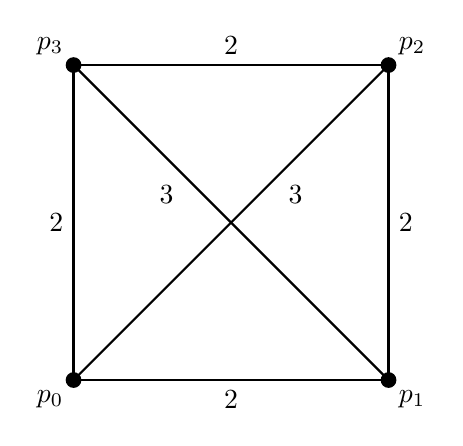
\begin{tikzpicture}[>=latex,thick]
\def\r{2}
\fill (-\r,-\r) circle[radius=0.1];
\fill (-\r,+\r) circle[radius=0.1];
\fill (+\r,-\r) circle[radius=0.1];
\fill (+\r,+\r) circle[radius=0.1];
\draw (-\r,-\r) -- (+\r,-\r);
\draw (-\r,-\r) -- (-\r,+\r);
\draw (-\r,-\r) -- (+\r,+\r);
\draw (+\r,-\r) -- (-\r,+\r);
\draw (+\r,-\r) -- (+\r,+\r);
\draw (+\r,+\r) -- (-\r,+\r);
\node at (-\r,0) [left] {$2$};
\node at (+\r,0) [right] {$2$};
\node at (0,-\r) [below] {$2$};
\node at (0,+\r) [above] {$2$};
\node at ({-0.3*\r},{0.3*\r}) [below left] {$3$};
\node at ({0.3*\r},{0.3*\r}) [below right] {$3$};
\node at (-\r,-\r) [below left] {$p_0$};
\node at (+\r,-\r) [below right] {$p_1$};
\node at (-\r,+\r) [above left] {$p_3$};
\node at (+\r,+\r) [above right] {$p_2$};
\end{tikzpicture}
\caption{Eine unmögliche Konstellation von vier Punkten.
Die Unmöglichkeit kann mit Hilfe des Kriteriums von
Satz~\ref{satz:npunkte-mit-abstaenden} nachgewiesen werden.
\label{fig:4punkte-mit-abstaenden}}
\end{figure}

\begin{beispiel}
Kann man vier Punkte in $\mathbb R^3$ finden derart, dass sie die
Abstände gemäss Abbildung~\ref{fig:4punkte-mit-abstaenden} haben?

Die Dreiecksungleichung ist nirgends verletzt, daran kann es also nicht liegen.
Da die Diagonale eines Quadrates  mit Seitenlänge $2$ nur $2\sqrt{2} < 3$ und
damit kürzer ist also verlangt, ist eine Lösung in der Ebene sicher nicht 
möglich.
Aber wenn man die dritte Dimension nutzen will ist das nur möglich, indem man
die Verbindungen zwischen diagonalen Punkten weiter verkürzt.

Dieses Argument ist etwas ad hoc, wir berechnen daher die Matrix $G$
gemäss Satz~\ref{satz:npunkte-mit-abstaenden}.
Zunächst brauchen wir die Matrix $M$:
\[
M = 
\begin{pmatrix}
0&2&3&2\\
2&0&2&3\\
3&2&0&2\\
2&3&2&0
\end{pmatrix}.
\]
Daraus ergibt sich jetzt die Matrix
\[
G =
\begin{pmatrix}
             4&\frac12(4+9-4)&\frac12(4+4-9)\\
\frac12(4+9-4)&             9&\frac12(9+4-4)\\
\frac12(4+4-9)&\frac12(9+4-4)&             4
\end{pmatrix}
=
\frac12
\begin{pmatrix}
 8& 9&-1\\
 9& 9& 9\\
-1& 9& 4
\end{pmatrix}.
\]
Bei der Durchführung der Cholesky-Zerlegung findet man allerdings
\[
\begin{pmatrix}
 8& 9&-1\\
 9& 9& 9\\
-1& 9& 4
\end{pmatrix}
=
\begin{pmatrix}
2\sqrt{2}            &   0    & 0 \\
\frac{9}{2\sqrt{2}}  & l_{22} & 0 \\
-\frac{1}{2\sqrt{2}} &        &   
\end{pmatrix}
\begin{pmatrix}
2\sqrt{2} & \frac{9}{2\sqrt{2}} & -\frac{1}{2\sqrt{2}} \\
0         &     l_{22}          &                      \\
0         &            0        &         
\end{pmatrix}
\]
wobei für $l_{22}$ die Gleichung
\[
9
=
l_{22}^2 + \biggl(\frac{9}{2\sqrt{2}}\biggr)^2
=
l_{22}^2 + \frac{81}{8}
=
l_{22}^2 + 10.125
\qquad\Rightarrow\qquad
l_{22}^2 = -\frac{7}{8} < 0
\]
gelten muss, die in $\mathbb{R}$ nicht erfüllbar ist.
Daraus schliess man, dass $G$ nicht positiv definit sein kann.

In diesem niedrigdimensionalen Fall kann man die Eigenschaft, dass
$G$ nicht positiv definit ist, auch mit Hilfe der Determinante erkennen.
Eine Gram-Determinante ist immer positiv, aber $\det(G)<0$.
Für grosse $n$ ist die Berechnung der Determinanten eher aufwendiger
als die Berechnung der Cholesky-Zerlegung.
\end{beispiel}

Aus dieser Lösung der geometrischen Aufgabe können wir noch mehr lernen.
Eine $n\times n$-Matrix kann nur dann die Gram-Matrix von $n$ Vektoren
$p_1,\dots,p_n\in\mathbb{R}^N$
sein, wenn sie positiv definit ist.
Positiv Definitheit kann man natürlich prüfen, indem man die
Cholesky-Zerlegung $G=LL^t$ findet.
Ausserdem können wir dann immer eine orthonormierte Basis
$b_1,b_2,\dots,b_N$ finden, so dass
\begin{align*}
p_1&=l_{11} b_1,
\\
p_2&=l_{21} b_1 + l_{22} b_2,
\\
p_3&=l_{31} b_1 + l_{32} b_2 + l_{33} b_3
\\
&\quad\vdots
\\
p_n&=l_{n1} b_1 + l_{n2} b_2 + l_{n3} b_3 + \dots + l_{nn} b_n.
\end{align*}
Die Matrix $L^t$ ist also auch die Matrix $R$ einer QR-Zerlegung der Matrix
der Vektoren, deren Gram-Matrix $G$ ist.
